\documentclass[UTF8,a4paper,11pt,fontset=windows]{ctexart}
\usepackage[a4paper,top=20mm,bottom=18mm,left=18mm,right=18mm,headheight=22pt]{geometry}
\usepackage{amsmath,amssymb,graphicx,booktabs,tabularx,longtable,seqsplit}
\usepackage[table]{xcolor}
\usepackage{enumitem,titlesec,fancyhdr,hyperref,url,tcolorbox,caption,float,microtype}
\definecolor{DeepInk}{HTML}{19313B}
\definecolor{Teal}{HTML}{0F6B67}
\definecolor{Coral}{HTML}{D4664A}
\definecolor{SoftGray}{HTML}{F3F6F5}
\definecolor{MidGray}{HTML}{67757B}
\definecolor{RuleGray}{HTML}{D7DEDC}
\hypersetup{colorlinks=true,linkcolor=Teal,urlcolor=Coral,pdftitle={BM3R1驱动的sRNA Shutdown模块建模报告}}
\setlength{\parindent}{2em}
\setlength{\parskip}{0.3em}
\setlist[itemize]{leftmargin=2em,itemsep=0.15em}
\setlist[enumerate]{leftmargin=2.2em,itemsep=0.2em}
\renewcommand{\arraystretch}{1.16}
\captionsetup{font=small,labelfont={bf,color=Teal},skip=5pt}
\titleformat{\section}{\Large\bfseries\color{DeepInk}}{\thesection.}{0.5em}{}
\titleformat{\subsection}{\large\bfseries\color{Teal}}{\thesubsection}{0.5em}{}
\pagestyle{fancy}
\fancyhf{}
\fancyhead[L]{\small\color{MidGray}BM3R1驱动的sRNA Shutdown模块建模报告}
\fancyhead[R]{\small\color{MidGray}版本 3.3}
\fancyfoot[C]{\small\color{MidGray}\thepage}
\renewcommand{\headrulewidth}{0.4pt}
\newcolumntype{Y}{>{\raggedright\arraybackslash}X}
\newtcolorbox{boundarybox}{colback=SoftGray,colframe=Teal,boxrule=0.7pt,arc=1.5mm,left=3mm,right=3mm,top=2mm,bottom=2mm}

\begin{document}
\begin{titlepage}
\thispagestyle{empty}
\vspace*{15mm}
{\color{Teal}\rule{25mm}{2.2pt}}\\[7mm]
{\fontsize{25}{31}\selectfont\bfseries\color{DeepInk}BM3R1驱动的sRNA\\[2mm]Shutdown模块建模报告}\\[7mm]
{\large\color{MidGray}方程纠正、参数溯源与转录供给可行域分析}\\[10mm]
\begin{tabular}{@{}ll@{}}
  \textbf{版本} & 3.3（参数底层来源与单/多bit解释修正版）\\
\textbf{日期} & 2026-09-09\\
\textbf{研究性质} & 确定性ODE建模与条件性参数分析
\end{tabular}
\vspace{11mm}
\begin{tcolorbox}[colback=DeepInk,colframe=DeepInk,arc=1.5mm,boxrule=0pt,left=5mm,right=5mm,top=4mm,bottom=4mm]
{\color{white}\bfseries 核心结果}\\[2mm]
  {\color{white}修正后的sRNA与mRNA共同降解方程采用Levine等人的RyhB/sodB参数代理。当前单bit基准中，新生输出FWHM由10.61 h缩短至6.98 h，LR后期产生由峰值97.9\%降至17.0\%。10.61 h不是多bit系统的表达上限；Shutdown的意义是使输出无需等待DNA状态改变即可自行关闭。}
\end{tcolorbox}
\vfill
  {\small\color{MidGray}本报告不代表wet-lab验证；已选RyhB参考序列，但ODE并非逐碱基模型，且输出蛋白仍未指定。}
\end{titlepage}

\section*{摘要}
本研究建立“振荡器--$\phi$C31/RDF计数器--BM3R1/sRNA Shutdown”耦合模型。本版明确采用\textit{E. coli} K-12 RyhB参考序列，补齐换算参数的原始数值、论文位置与底层实验来源，并改用逐条件无Shutdown对照。50 min倍增时间下，当前单bit测试中Shutdown保留98.6\%输出峰值，将新生输出FWHM由10.61 h压缩至6.98 h，并保持5/5周期一次输入一次完整反转。多bit译码可能让无Shutdown输出跨越多个输入周期，因此10.61 h不是完整系统的上限。序列本身不进入ODE，故结论仍为机制级预测。

\begin{boundarybox}
\textbf{结论边界：}结果支持“在特定、可解释参数区域内机制可行”，不支持“已经实验验证”或“具有99.2\%成功率”。
\end{boundarybox}

\begin{boundarybox}
\textbf{单bit与多bit：}当前bit每次输入就在PB和LR之间交替，无Shutdown对照只覆盖约一个LR驻留间隔。若目标译码状态连续$m$个输入周期保持有效，无Shutdown持续时间可近似随$mT_{\mathrm{input}}$增长，可能远长于10.61 h。准确数值须等实验组确定计数位、目标状态与复位逻辑后再计算。
\end{boundarybox}

\section{模型范围与上游接口}
计数器直接加载\nolinkurl{rdfmodel_new/model/zhao_core.py}的38状态$\phi$C31 integrase/RDF网络。振荡器向计数器提供C31翻译通量：
\begin{equation}
v_{\mathrm{Int}}(t)=0.45v_{31}(t).
\end{equation}
名义接口采用C31 RBS scale 0.45、Integrase标签损失率8 h$^{-1}$和50 min倍增时间。Zhao等人的文献支持反应网络与延迟抑制器结构；当前BM3R1和RDF表达参数是\nolinkurl{rdfmodel_new}筛选的工程工作点，不是Zhao原文常数。双初态最低P score为0.99526，5个稳定周期均恰好一次完整反转。

\begin{figure}[H]\centering
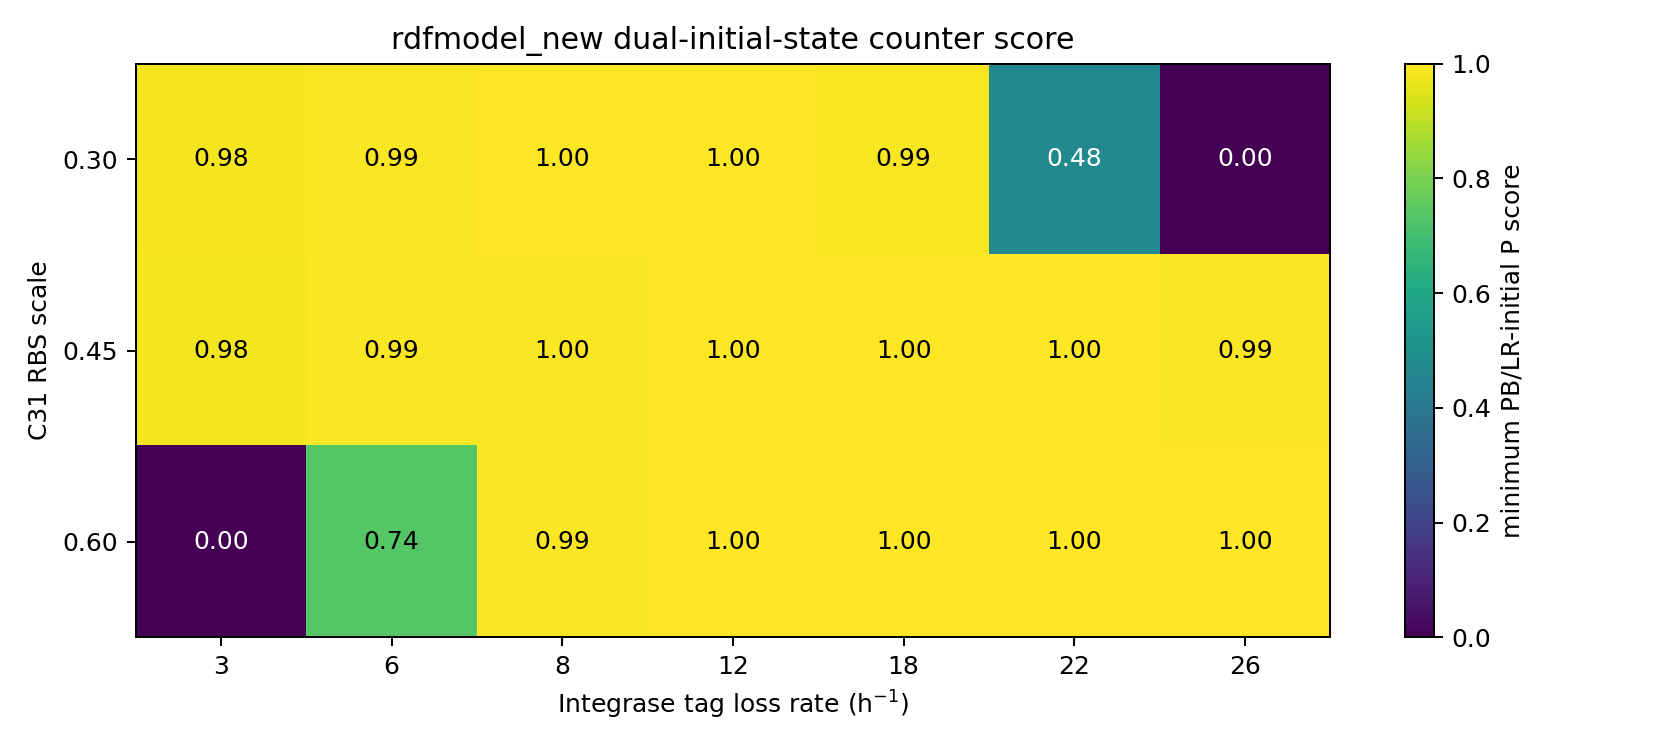
\includegraphics[width=0.79\textwidth]{assets/00_interface_scan_heatmap.png}
\caption{\nolinkurl{rdfmodel_new}的C31 RBS/Integrase标签双初态接口审计。}
\end{figure}

\section{纠正后的Shutdown方程}
PB状态表达BM3R1并抑制Shutdown promoter；PB转为LR后，BM3R1下降，Shutdown promoter解除抑制并产生靶向输出mRNA的sRNA。新增状态为sRNA $S$、输出mRNA $M$和归一化蛋白$O$。

\begin{align}
H(B)&=\ell+(1-\ell)\frac{1}{1+[B/(r_KK_{\mathrm{RDF}})]^n},\\
\frac{dS}{dt}&=\alpha_SH(B)-\beta_SS-pkSM,\\
\frac{dM}{dt}&=\alpha_M f_{LR}-\beta_MM-kSM,\\
\frac{dO}{dt}&=\beta_{tr}M-(\delta_O+\mu)O.
\end{align}

$p=1$时，每个配对通量同时消耗一份sRNA和一份mRNA。这里$p=1$是Levine理论分析的一对一极限，不是实验直接辨识常数；扩展分析扫描$p=0.5$--1。旧版遗漏$S$方程中的$-pkSM$，会夸大sRNA积累和关闭能力。$\beta_S$、$\beta_M$按Levine文献中的有效RNA周转率处理，不再额外叠加稀释；蛋白仍包含生长稀释。

\section{参数来源与证据等级}
\subsection{文献锚定参数}
{\footnotesize
\begin{longtable}{@{}p{0.13\textwidth}p{0.14\textwidth}p{0.27\textwidth}p{0.38\textwidth}@{}}
\caption{RyhB/sodB代理参数、单位换算与底层来源}\\
\toprule
参数 & 模型值 & 文献原值与换算 & 直接来源及底层依据\\
\midrule
\endfirsthead
\toprule
参数 & 模型值 & 文献原值与换算 & 直接来源及底层依据\\\midrule
\endhead
$\alpha_M$ & 基准0.03；扫描0.006--0.06 $\mu$M/h & 基准0.5 nM/min：$0.5\times60/1000=0.03$；扫描0.1--1同理换算 & Levine由约10--20 copies/cell估计表达态约1 nM/min；底层转录组为Zhang 2005与Selinger 2000\\
$\alpha_S$ & 基准0.06；扫描0.006--0.6 $\mu$M/h & 基准1 nM/min：$1\times60/1000=0.06$；文献范围0.1--10 & Levine Figure 1C、Table 1和参数估计小节\\
$\beta_M$ & 6 h$^{-1}$ & 约6 min sodB半衰期对应Levine近似$1/10=0.1$ min$^{-1}$；$0.1\times60=6$ & Levine参数估计小节；底层sodB实验为Massé 2003\\
$\beta_S$ & 1.2 h$^{-1}$ & Levine取$1/50\approx0.02$ min$^{-1}$；$0.02\times60=1.2$ & 约30 min RyhB半衰期依据Massé 2003与Moll 2003；沿用Levine近似率，不重算$\ln2/t_{1/2}$\\
$k$ & 1200 $\mu$M$^{-1}$h$^{-1}$ & $1/50=0.02$ nM$^{-1}$min$^{-1}$；$0.02\times1000\times60=1200$ & Levine根据Massé中RyhB约3 min内消失和靶mRNA约20 nM推得；非直接结合测量\\
$p$ & 基准1；扫描0.5--1 & 理论一对一极限；无单位换算 & Levine理论模型情形，非实验辨识常数\\
\bottomrule
\end{longtable}}

单位换算只改变数值表示，不提高证据等级。表中同时列出Levine的原始估计、其引用的底层实验和本项目选择的设计点。

基准取$\alpha_M=0.03$、$\alpha_S=0.06\ \mu$M/h，即0.5和1 nM/min。Levine对表达状态下的靶mRNA给出约1 nM/min量级并指出通常可变化约10倍，但未指定本报告采用的单侧0.1--1 nM/min区间；因此$\alpha_M=0.006$--0.06 $\mu$M/h是本项目声明的保守包络，不是文献直接区间。$\alpha_S=0.06$是Levine计算使用的参考量级而非文献上限，并满足基准下一对一共同降解的供给要求。核查点$\alpha_S=\alpha_M=0.03$时，LR后期仍残留38.3\%，未通过关闭标准。

\subsection{RyhB序列与适用边界}
本模型采用\textit{E. coli} K-12 MG1655 RyhB（NCBI Gene 2847761，locus \nolinkurl{b4451}）。NCBI当前注释为\nolinkurl{NC_000913.3 complement(3580922..3581016)}，长度95 nt：

\begin{center}
\begin{minipage}{0.96\textwidth}\small\ttfamily\raggedright
DNA 5'-\seqsplit{GCGATCAGGAAGACCCTCGCGGAGAACCTGAAAGCACGACATTGCTCACATTGCTTCCAGTATTACTTAGCCAGCCGGGTGCTGGCTTTTTTTTT}-3'\\[1mm]
RNA 5'-\seqsplit{GCGAUCAGGAAGACCCUCGCGGAGAACCUGAAAGCACGACAUUGCUCACAUUGCUUCCAGUAUUACUUAGCCAGCCGGGUGCUGGCUUUUUUUUU}-3'
\end{minipage}
\end{center}

Levine实验记载的克隆边界为RyhB $+1$到$+96$，但原文未打印完整96 nt insert序列；因此本报告不把当前95 nt feature之外的碱基擅自写成确定的成熟RNA。Hao等人指出RyhB的核心互作区、Hfq相关linker和终止结构均具有序列功能，故不应把截短或突变体与当前$k$、$\beta_S$直接混用。

当前ODE不读取碱基序列，而是把序列、Hfq和RNase E作用折叠进固定$k$。其定量依据最接近Levine验证的\nolinkurl{sodB -1..+88}控制区（含前11个密码子）融合靶标。若以后更换靶序列，当前数值不能原样移植。RyhB还存在多个内源靶标；内源竞争和铁代谢扰动未建模，所以本报告将其定位为文献锚定机制原型，而非正交化最终元件。

Shin等人报告B3-BM3R1 gate的\mbox{$y_{min}=0.005$ RPU}、\mbox{$y_{max}=0.6$ RPU}和$n=3.1$。本模型采用$n=3.1$及归一化leak $0.005/0.6=0.00833$。其$K$以RPU表示，不能直接用于BM3R1浓度；因此Shutdown默认继承counter的BM3R1阈值，以无量纲$r_K$表达相对阈值。

\subsection{明确标注的假设}
\begin{table}[H]\centering\small
\caption{无直接构建标定参数及其理由}
\begin{tabularx}{\textwidth}{@{}YcYY@{}}
\toprule
参数 & 基准 & 类别 & 理由\\
\midrule
$r_K$ & 1 & 设计假设 & 复用RDF的BM3R1 operator，避免新增RPU到$\mu$M换算\\
Shutdown/counter拷贝比 & 1 & 设计假设 & 每个counter plasmid配置一个Shutdown cassette\\
operator化学计量 & 2 & 机制假设 & TetR家族同源二聚体，每个operator计两个单体等价物\\
输出翻译比例 & 1 h$^{-1}$ & 归一化约定 & 只缩放纵轴，不决定mRNA时间指标\\
蛋白主动降解 & 0 h$^{-1}$ & 报告蛋白假设 & 稳定GFP代理，仅由生长稀释清除\\
\bottomrule
\end{tabularx}
\end{table}

每次运行均输出\nolinkurl{00_parameter_provenance.csv}，逐项记录证据等级、来源、换算和理由。

\section{基准结果}
本节比较的是当前单bit轨迹。该bit每次输入就在PB和LR之间交替，所以无Shutdown输出只覆盖约一个LR驻留间隔；10.61 h不是完整多bit系统的最长表达时间。
\begin{table}[H]\centering
\caption{50 min倍增条件下的基准指标}
\begin{tabular}{@{}lrr@{}}\toprule
指标 & 单bit无Shutdown & 单bit文献锚定Shutdown\\\midrule
输出产生FWHM & 10.61 h & 6.98 h\\
LR后期输出产生/峰值 & 97.9\% & 17.0\%\\
输出产生峰值 & 0.004999 $\mu$M/h & 0.004930 $\mu$M/h\\
单次输出AUC & 0.0533 $\mu$M & 0.0372 $\mu$M\\
归一化蛋白FWHM & 10.63 h & 7.33 h\\
LR后期蛋白/峰值 & 99.8\% & 32.0\%\\
\bottomrule\end{tabular}
\end{table}

Shutdown使新生输出FWHM缩短34.2\%，将LR后期新生输出降低82.6\%，同时仅损失约1.4\%峰值。稳定蛋白下降慢于翻译通量，因为sRNA不清除已经合成的蛋白。

34.2\%只是同一单bit轨迹中的局部比较，不能代表多bit系统中Shutdown的全部收益。若完整计数逻辑使目标输出状态跨越$m$个输入间隔，无Shutdown持续时间可粗略写成$T_{\mathrm{no\ shutdown}}\sim mT_{\mathrm{input}}$，可能远长于10.61 h；$m$取决于尚未冻结的计数状态译码与复位逻辑。当前6.98 h是局部Shutdown动力学给出的关闭窗口。

\begin{figure}[H]\centering
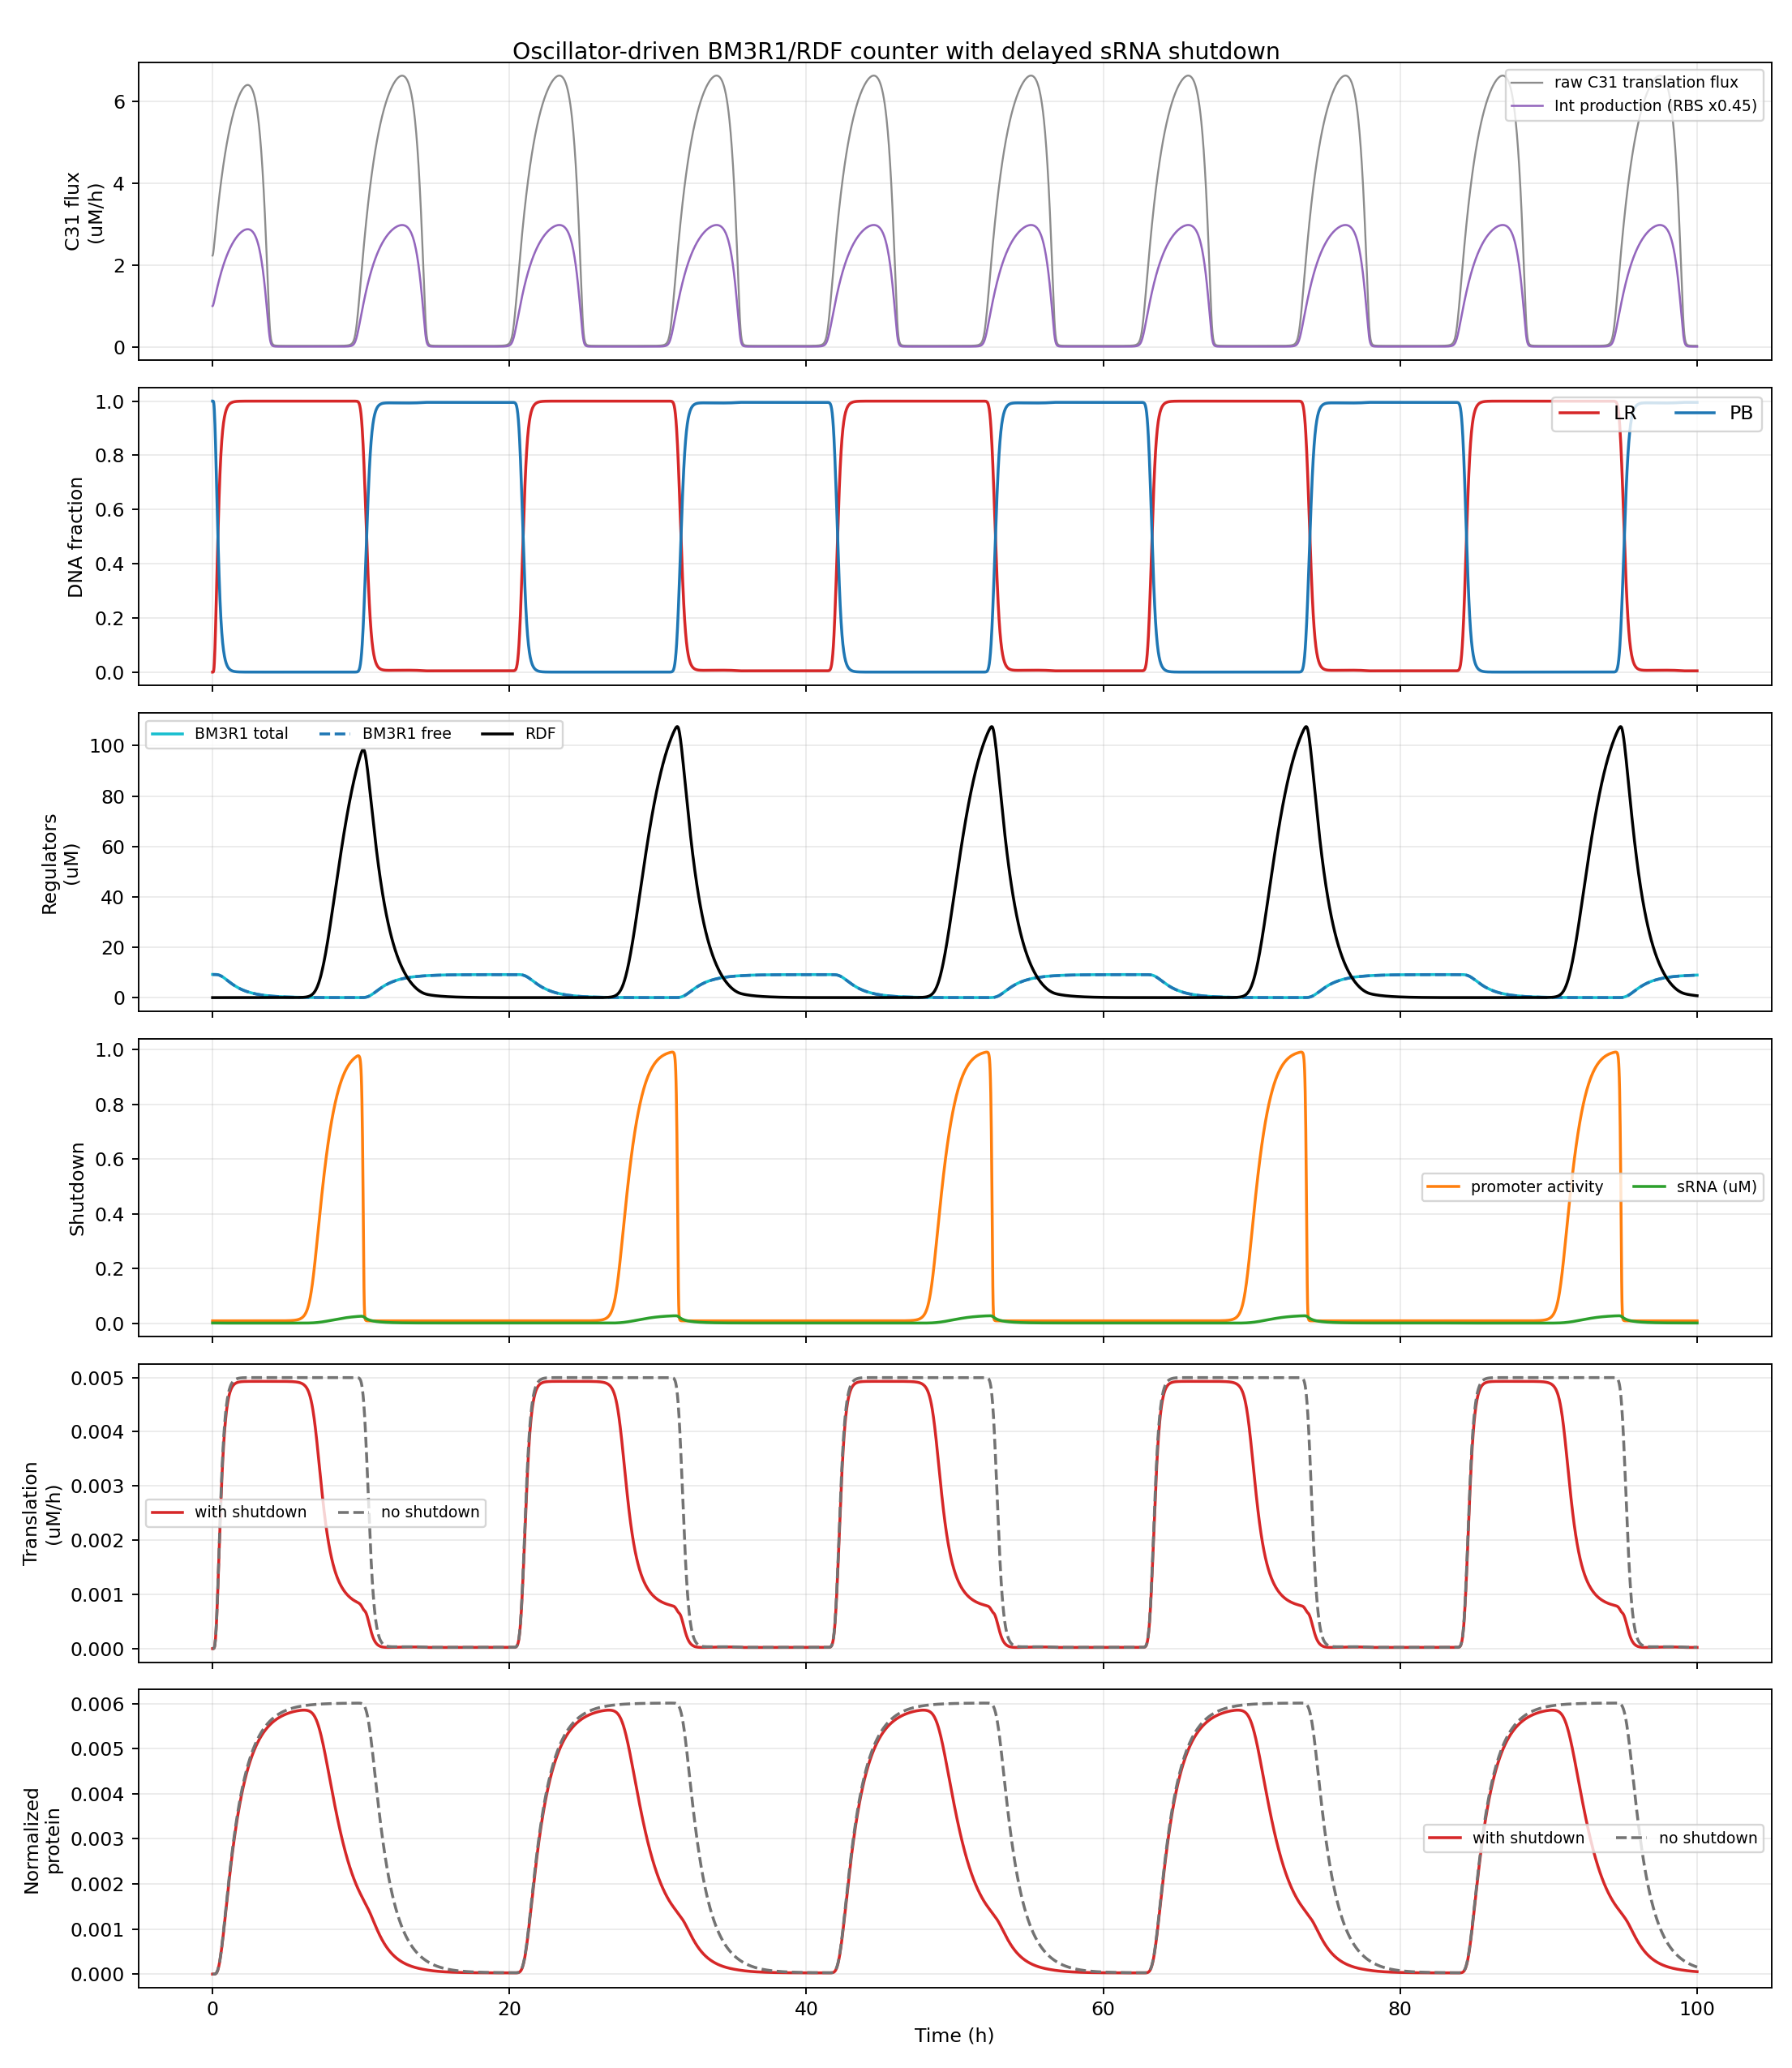
\includegraphics[width=0.94\textwidth]{assets/01_baseline_timecourse.png}
\caption{修正方程和文献参数下的完整耦合时间过程。}
\end{figure}

\section{可调性与可行域}
二维扫描采用Levine估计的$\alpha_S=0.006$--$0.6\ \mu$M/h量级和明示的$r_K=0.5$--2.0。工程标准为LR后期产生低于峰值20\%、峰值不低于对应无Shutdown对照50\%，这些阈值不是文献常数；扫描上限也不代表BM3R1 promoter已经过绝对标定。

169组中91组通过，FWHM为5.42--7.36 h。固定$r_K=1$时$\alpha_S$与脉宽、固定$\alpha_S=0.06$时阈值比与脉宽的Spearman相关系数均为$-1.000$；这些是单参数切片的单调关系，不是全局独立效应量。

\begin{figure}[H]\centering
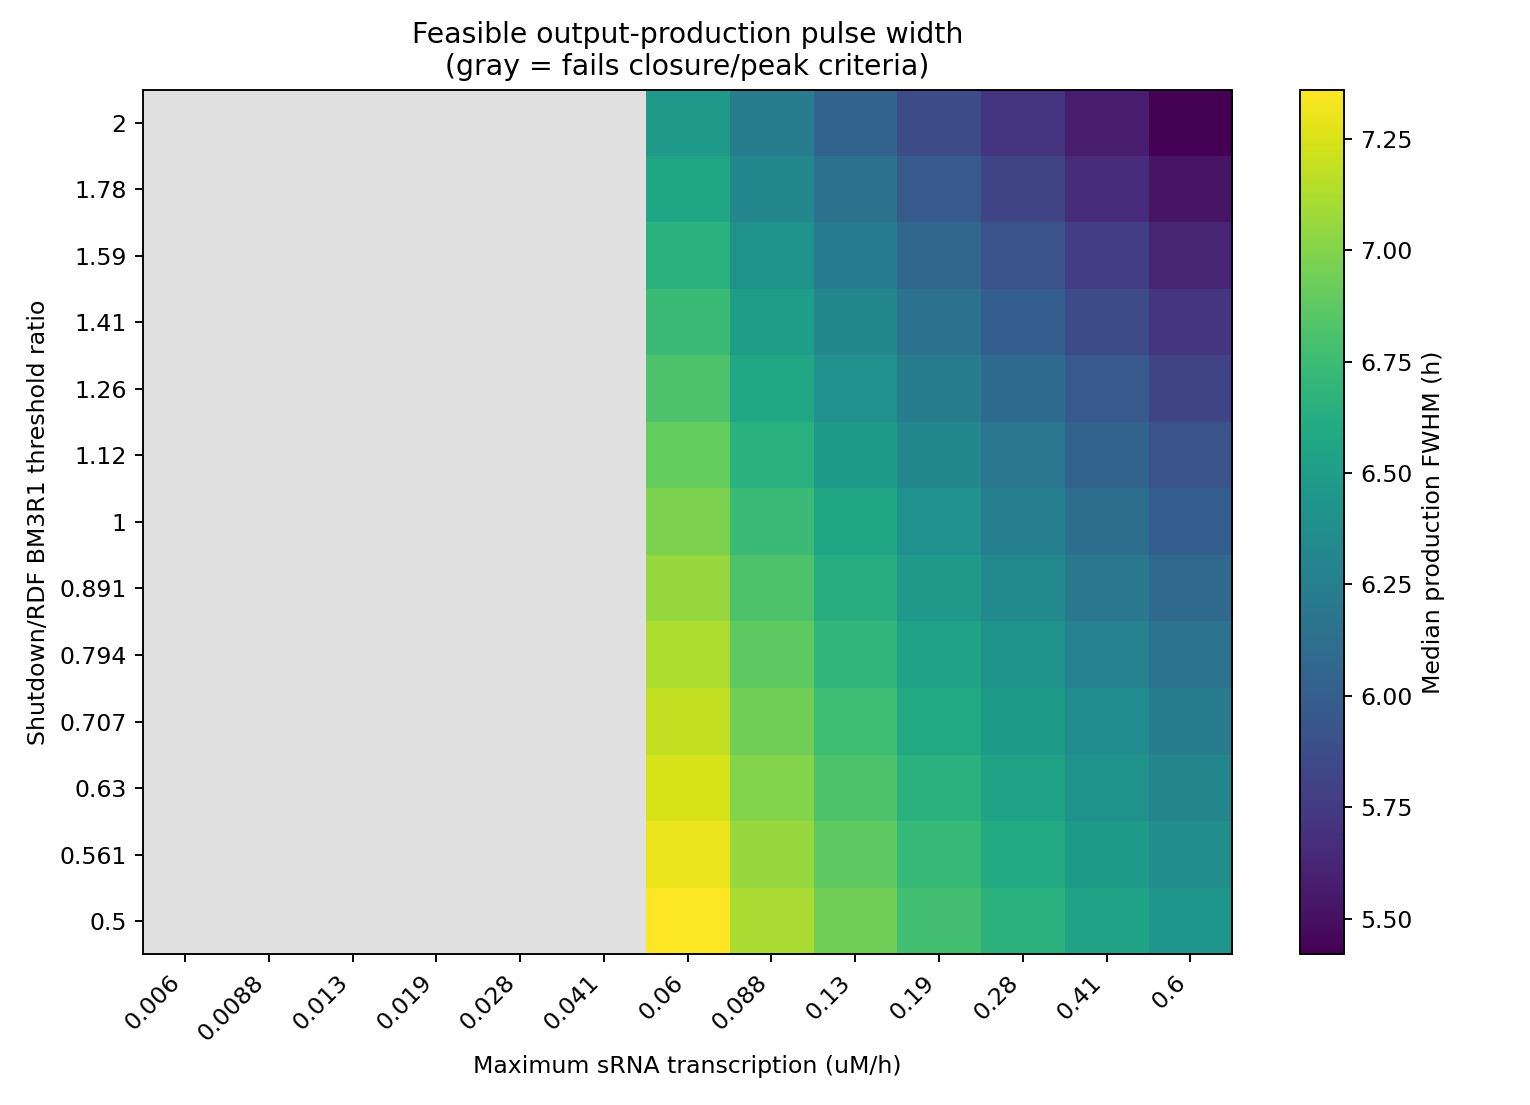
\includegraphics[width=0.75\textwidth]{assets/02_tunability_heatmap.png}
\caption{sRNA最大转录率和BM3R1相对阈值的可调性扫描。灰色区域未通过工程标准。}
\end{figure}

为直接检验共同降解的供给约束，模型扫描$\alpha_S=0.006$--0.6和$\alpha_M=0.006$--0.06 $\mu$M/h，并为每个$\alpha_M$单独计算无Shutdown峰值。225组中124组通过，15/15个靶转录水平存在可行解。离散网格最低可行供给比为1.39；边界中位数为2.68，最高为7.20。这些是当前轨迹、网格和$p=1$下的经验边界。

\begin{figure}[H]\centering
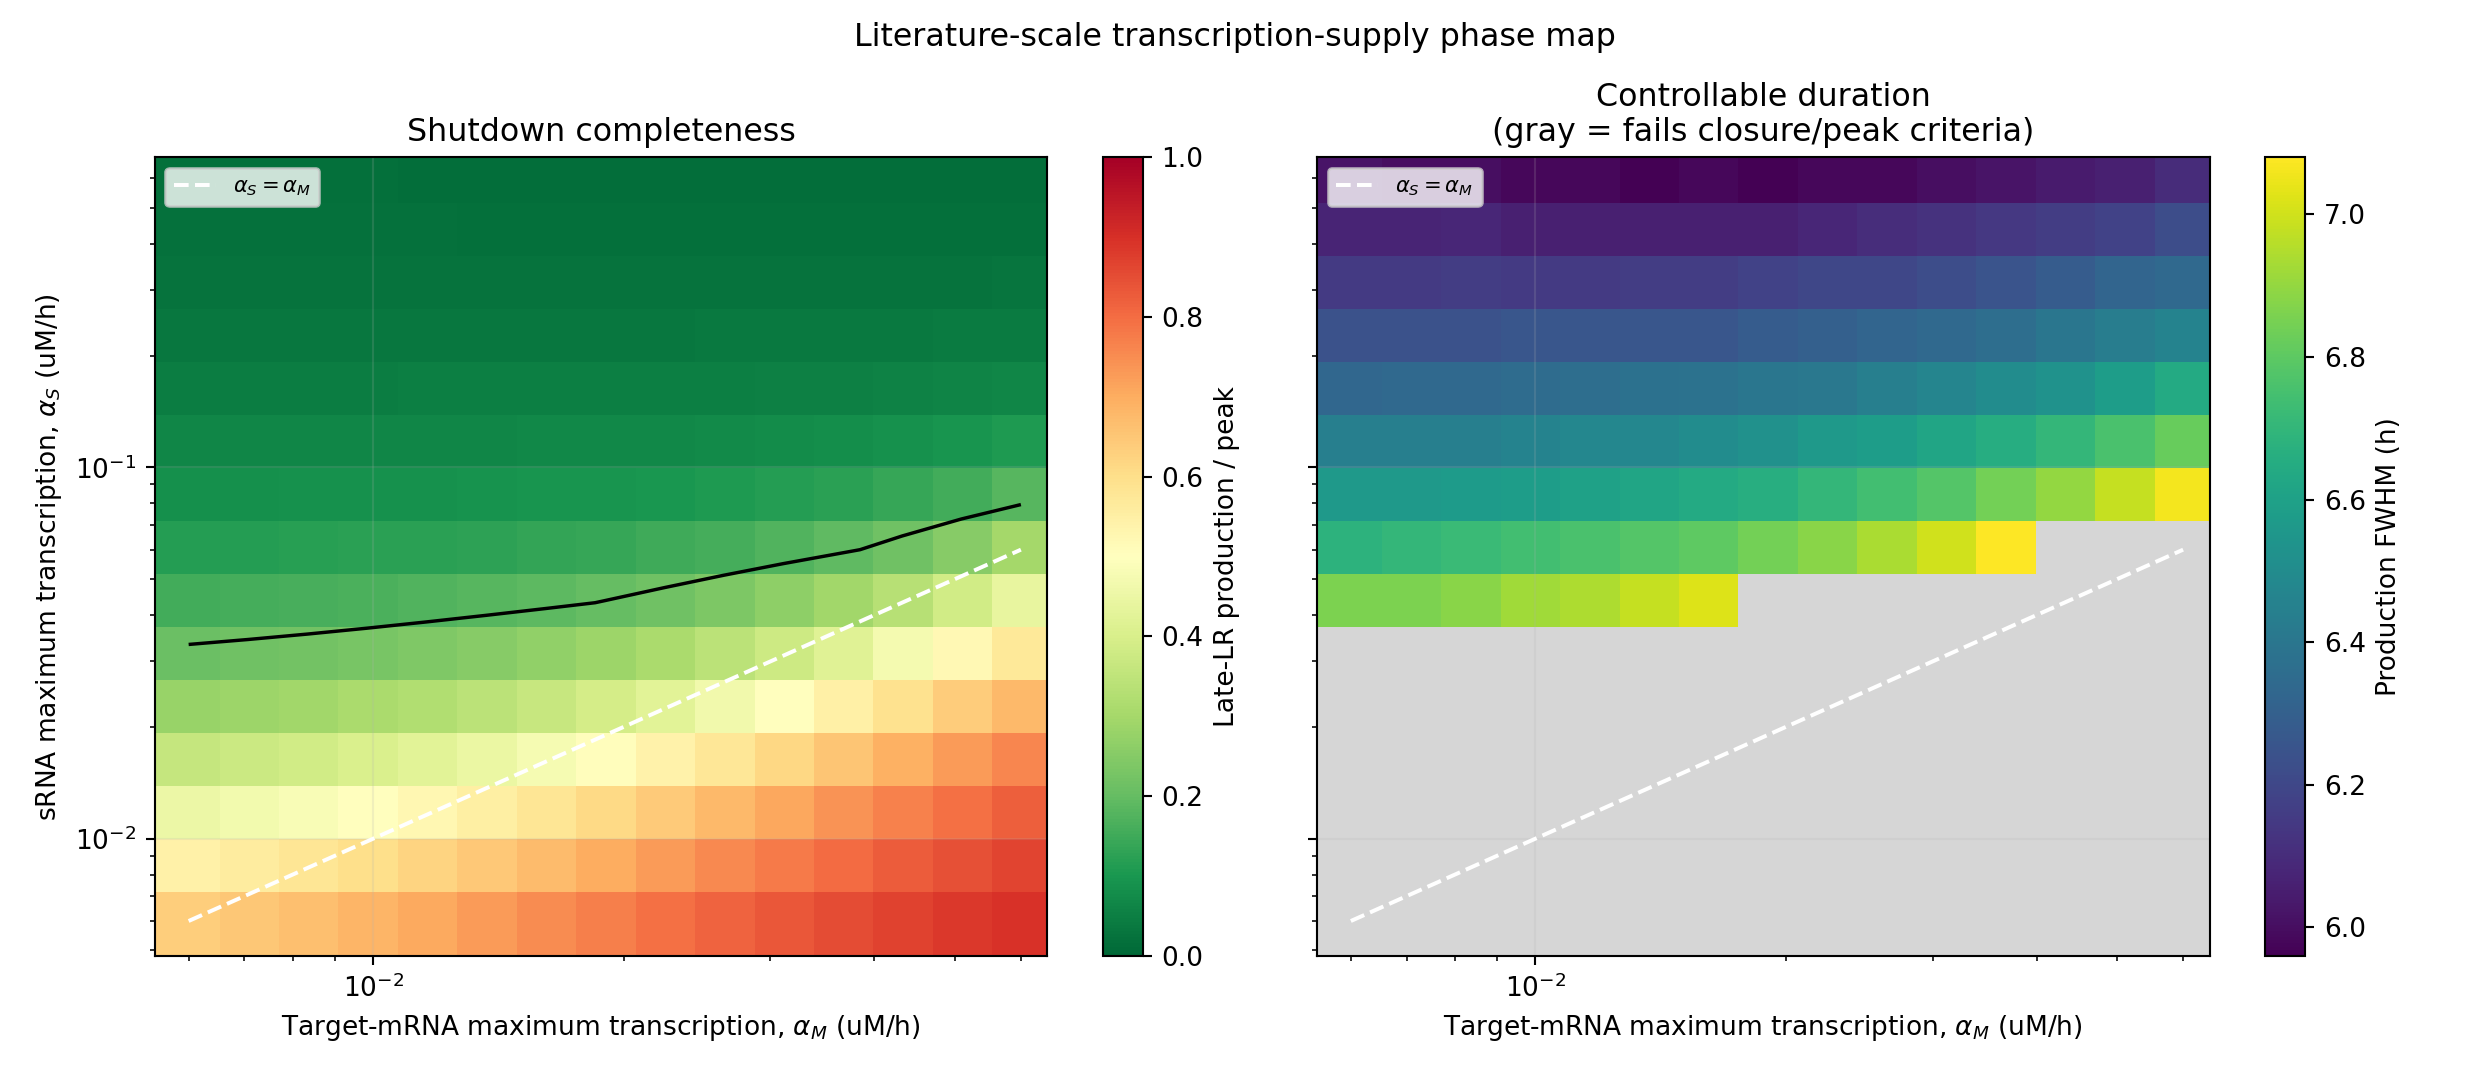
\includegraphics[width=0.98\textwidth]{assets/04_transcription_balance_phase_map.png}
\caption{转录供给相图。左图黑线为20\%关闭边界，右图灰色为未同时满足关闭与峰值标准的区域；白色虚线表示$\alpha_S=\alpha_M$。}
\end{figure}

\begin{figure}[H]\centering
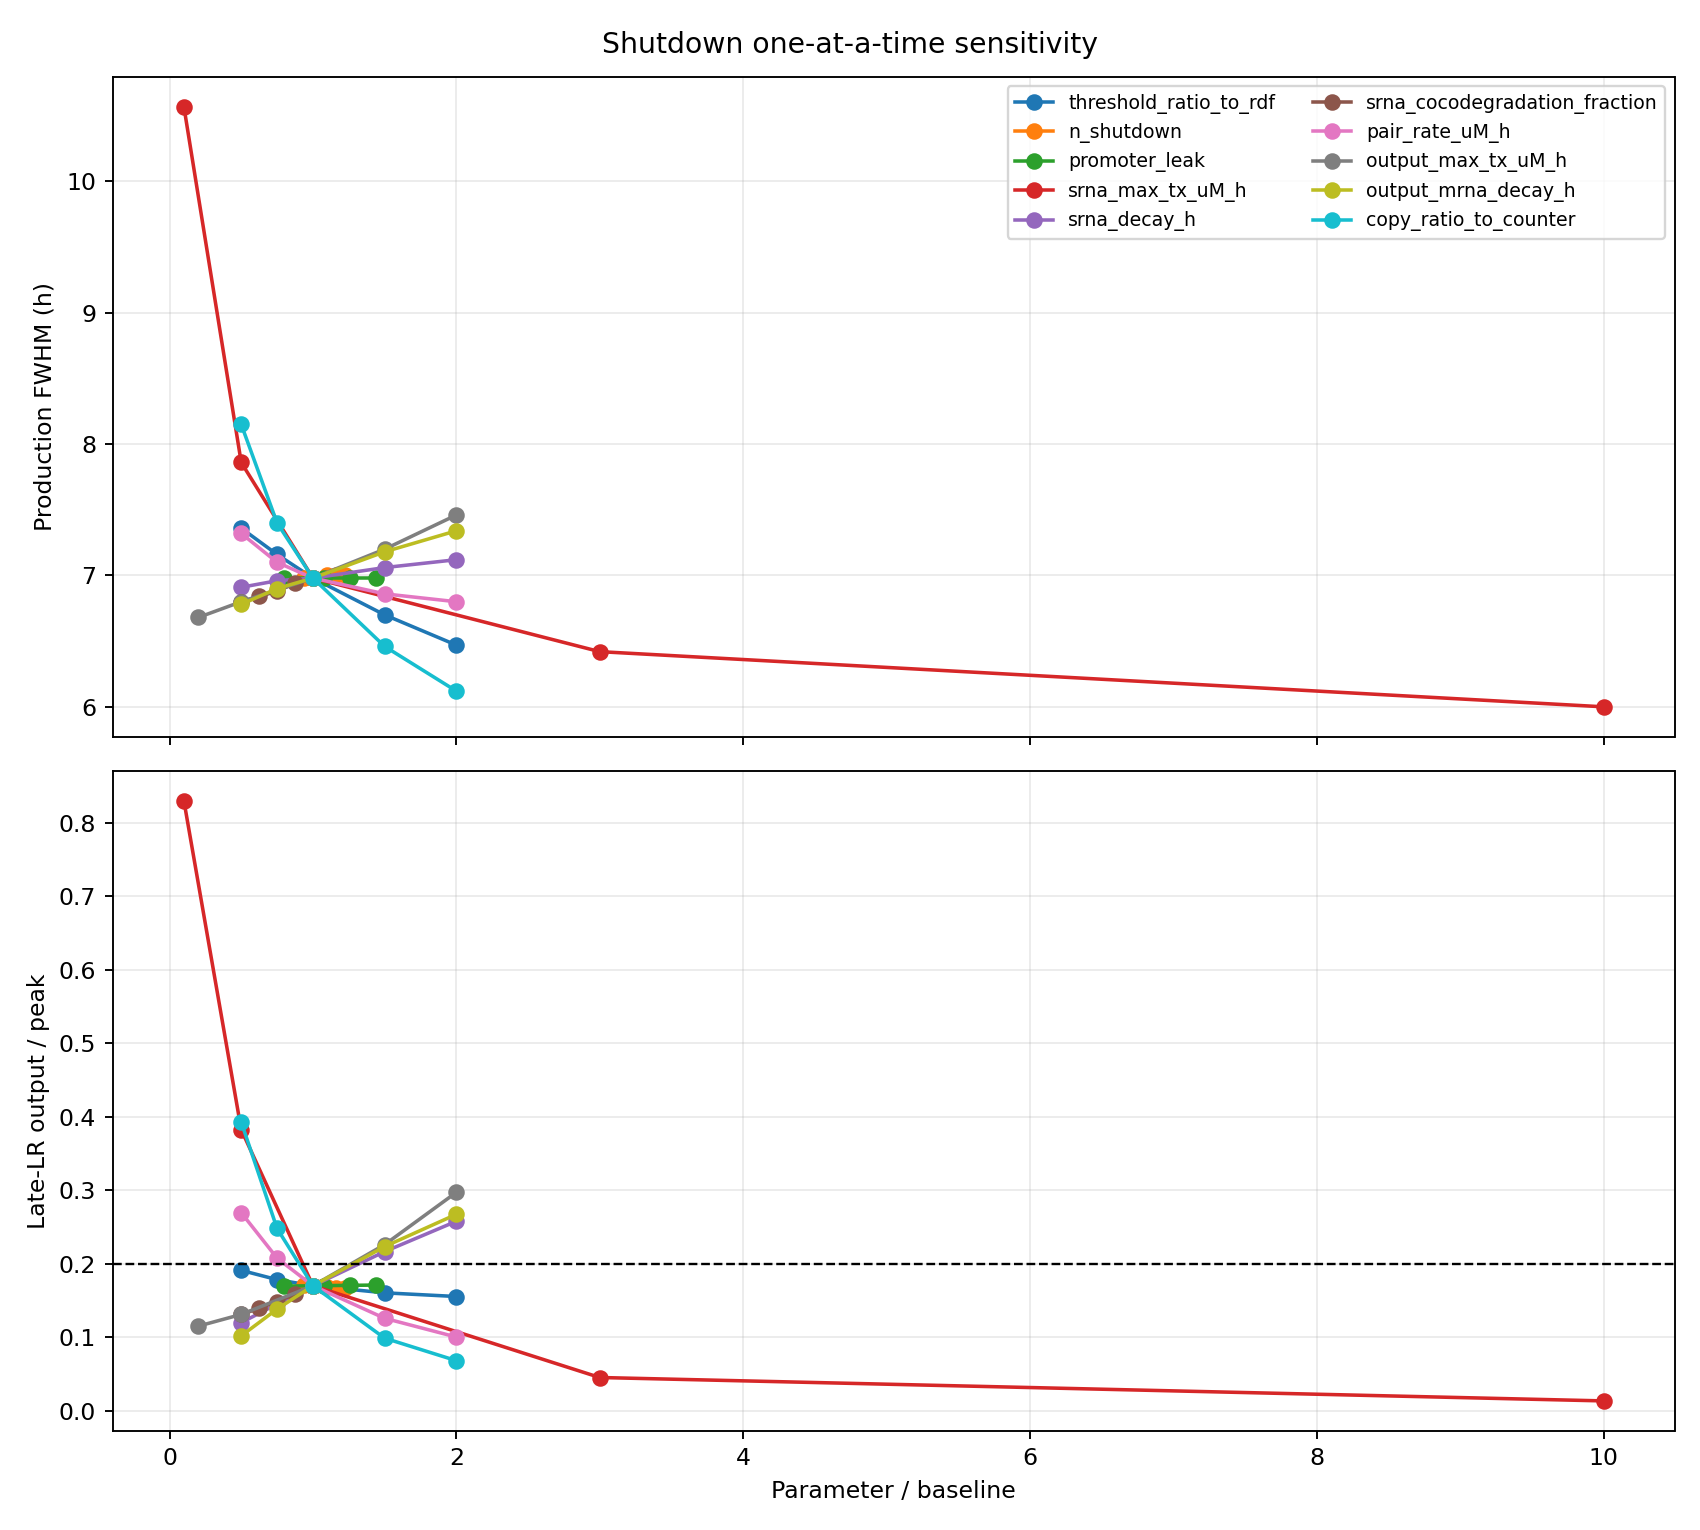
\includegraphics[width=0.79\textwidth]{assets/06_shutdown_oat_sensitivity.png}
\caption{文献量级与明示工程包络内的单参数敏感性。}
\end{figure}

\section{参数包络结果}
512点拉丁超立方抽样包含Levine估计的RNA量级、Shin BM3R1 Hill/leak值及声明的构建背景包络。每个样本采用与其靶mRNA转录率匹配的无Shutdown峰值对照。参数被独立组合，故该分析不保留真实构建中的参数相关性，也不是实验后验分布。

\begin{table}[H]\centering
\begin{tabular}{@{}lr@{}}\toprule
指标 & 结果\\\midrule
达到工程标准 & 277/512（54.1\%）\\
脉宽5\%/50\%/95\%分位数 & 5.70/6.86/10.54 h\\
LR后期残留95\%分位数 & 77.9\%\\
通过/失败样本有效供给比中位数 & 8.41/0.86\\
首要宽度与关闭参数 & sRNA最大转录率\\
\bottomrule\end{tabular}
\end{table}

有效供给比定义为$\alpha_SC/\alpha_M$，$C$为cassette剂量比。供给比低于1时2.3\%通过，1--2时23.0\%，2--4时61.3\%，4--8时91.7\%，不低于8时89.0\%。高供给端有少量峰值损失，但当前BM3R1延迟通常保留脉冲前段。54.1\%仅是声明包络的覆盖率，对上下限和抽样尺度敏感，不是wet-lab成功概率。

\begin{figure}[H]\centering
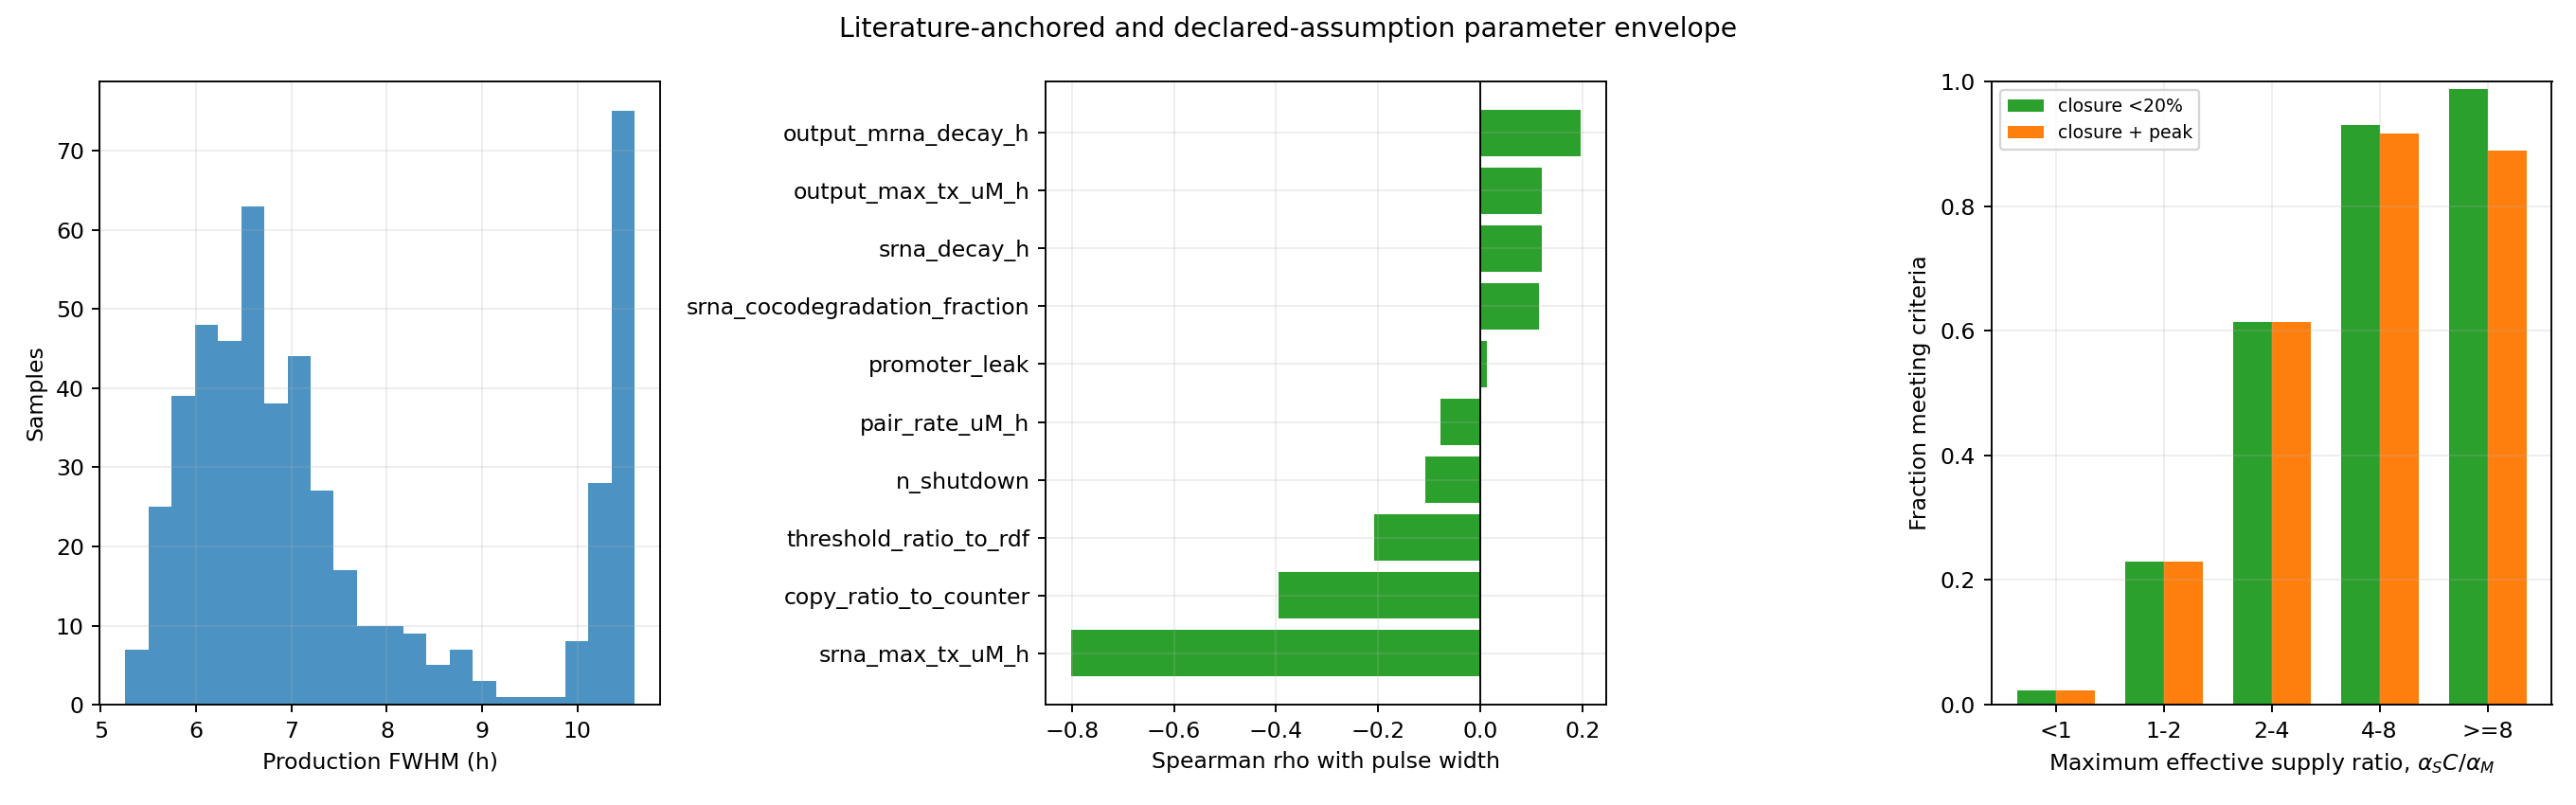
\includegraphics[width=0.85\textwidth]{assets/07_shutdown_joint_uncertainty.png}
\caption{512点拉丁超立方联合包络。右图区分关闭完整度和关闭加峰值的联合标准。}
\end{figure}

\section{Operator负载与生长条件}
基准拷贝比为1时，快速平衡模型估算最低游离BM3R1为总量的50.6\%。计数器P score由0.995260变为0.995278，5/5周期仍一次完整反转。将拷贝比扫描至10时计数评分也未下降，但这只是当前负载模型的压力测试，不能替代真实拷贝数与结合常数。

\begin{figure}[H]\centering
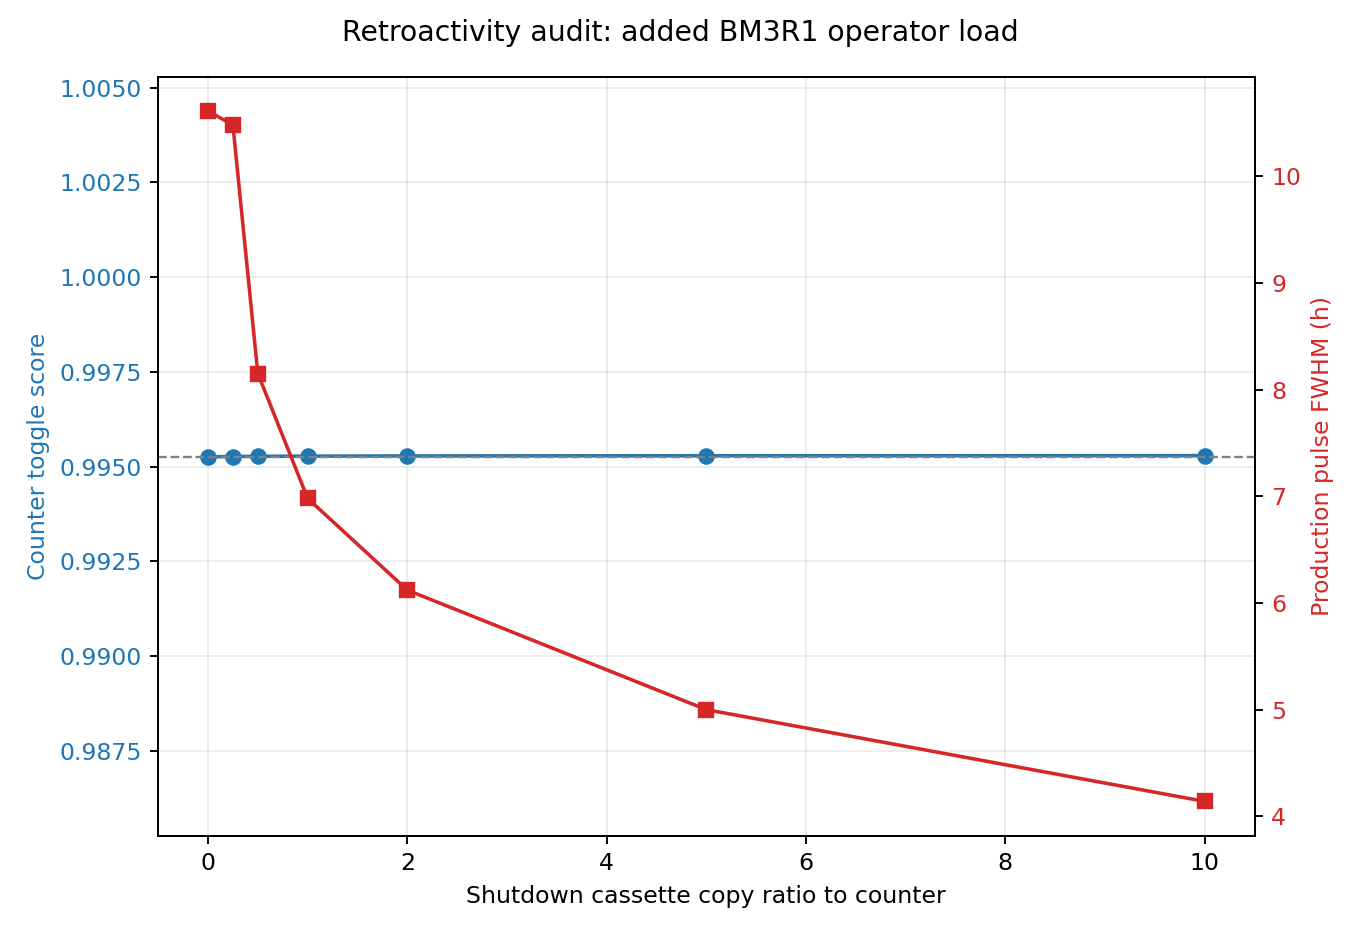
\includegraphics[width=0.76\textwidth]{assets/03_operator_load_audit.png}
\caption{Shutdown cassette剂量对计数器评分与输出时长的影响。}
\end{figure}

\begin{table}[H]\centering\small
\caption{自洽生长速度分析}
\begin{tabular}{@{}rrrrrr@{}}\toprule
倍增时间 & 振荡周期 & 产生FWHM & 后期产生 & 后期蛋白 & 一峰一次反转\\\midrule
40 min & 7.97 h & 5.48 h & 19.1\% & 39.0\% & 100\%\\
50 min & 10.59 h & 6.98 h & 17.0\% & 32.0\% & 100\%\\
60 min & 13.34 h & 8.54 h & 16.1\% & 27.9\% & 100\%\\
\bottomrule\end{tabular}
\end{table}

\begin{figure}[H]\centering
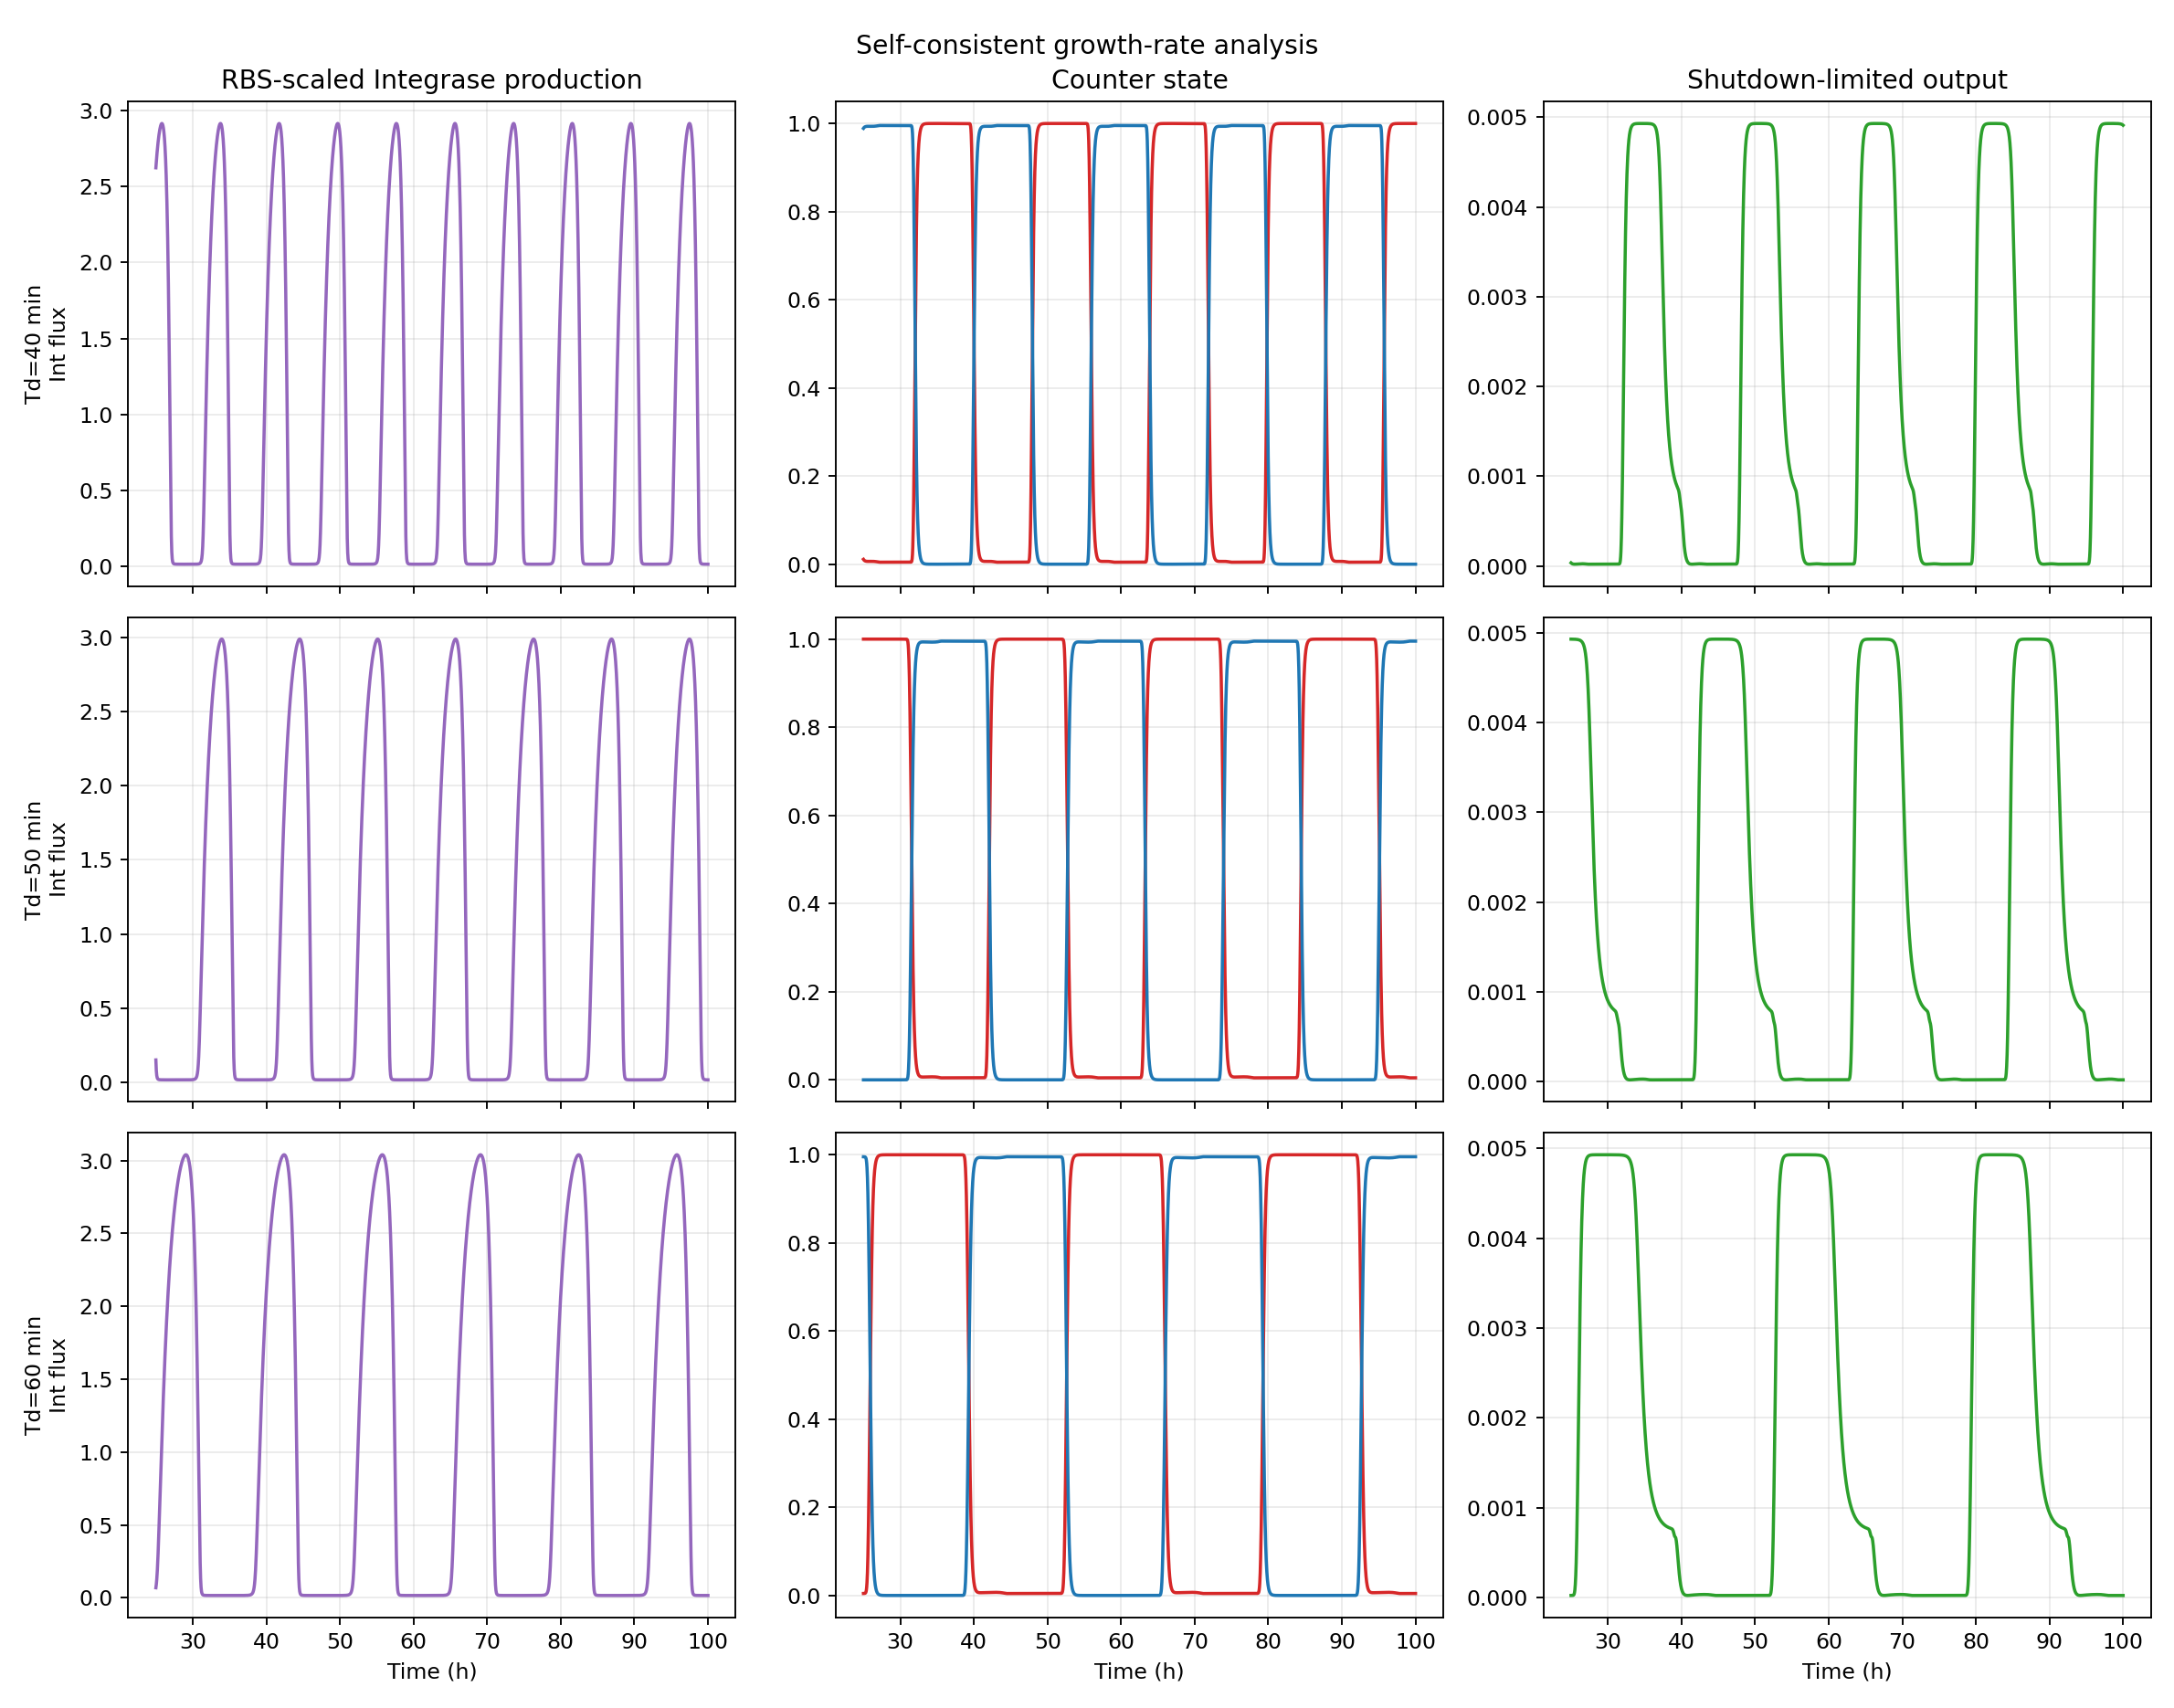
\includegraphics[width=0.89\textwidth]{assets/05_self_consistent_growth.png}
\caption{40、50和60 min倍增条件下自洽重算的输入、计数状态与Shutdown输出。}
\end{figure}

三种条件均使用各自无Shutdown峰值作对照并能停止新的输出产生，但稳定蛋白存量没有同步降到20\%以下。若最终功能要求蛋白浓度快速下降，应指定输出蛋白并加入有文献半衰期的降解标签。

\section{结论与下一步}
\begin{enumerate}
\item 修正后的共同降解方程与Levine模型一致，配对通量同时消耗mRNA和sRNA；
\item RyhB/sodB参数代理下，BM3R1下降能够把持续LR表达转成有限的新生输出脉冲；
\item 基准FWHM约6.98 h、LR后期产生约17.0\%，但这是条件性结果；
\item 表达时间可由sRNA转录率和BM3R1阈值调节，修正范围后91/169点通过，脉宽为5.42--7.36 h；
\item 离散网格最低可行$\alpha_S/\alpha_M$约为1.39，边界中位数约为2.68；512点声明包络有54.1\%通过，供给比仍是首要约束；
\item 当前负载模型未破坏一次输入一次反转，但拷贝数与负载仍需构建特异标定；
\item sRNA关闭新生翻译，不保证稳定蛋白同步消失。
\end{enumerate}

下一步应先明确是否采用与RyhB配套的\nolinkurl{sodB -1..+88}靶向接口，并检查融合边界的RNA结构；随后可扩展Hfq容量、内源靶标竞争及BM3R1 promoter的RPU到RyhB转录率映射。输出蛋白可以继续后置。

\section*{参考文献}
\begin{enumerate}[label={[\arabic*]}]
\item Zhao, J. et al. A single-input binary counting module based on serine integrase site-specific recombination. \textit{Nucleic Acids Research} 47, 4896--4909 (2019). \url{https://doi.org/10.1093/nar/gkz245}
\item Levine, E. et al. Quantitative characteristics of gene regulation by small RNA. \textit{PLoS Biology} 5, e229 (2007). \url{https://doi.org/10.1371/journal.pbio.0050229}
\item Shin, J. et al. Programming Escherichia coli to function as a digital display. \textit{Molecular Systems Biology} 16, e9401 (2020). \url{https://doi.org/10.15252/msb.20199401}
\item Potvin-Trottier, L. et al. Synchronous long-term oscillations in a synthetic gene circuit. \textit{Nature} 538, 514--517 (2016). \url{https://doi.org/10.1038/nature19841}
\item Hao, Y. et al. Quantifying the sequence--function relation in gene silencing by bacterial small RNAs. \textit{PNAS} 108, 12473--12478 (2011). \url{https://doi.org/10.1073/pnas.1100432108}
\item Massé, E. et al. Coupled degradation of a small regulatory RNA and its mRNA targets in \textit{Escherichia coli}. \textit{Genes \& Development} 17, 2374--2383 (2003). \url{https://doi.org/10.1101/gad.1127103}
\item Prévost, K. et al. Small RNA-induced mRNA degradation achieved through both translation block and activated cleavage. \textit{Genes \& Development} 25, 385--396 (2011). \url{https://doi.org/10.1101/gad.2001711}
\item NCBI Gene. \textit{ryhB} [\textit{E. coli} K-12 MG1655], Gene ID 2847761. \url{https://www.ncbi.nlm.nih.gov/gene/2847761}
\item Zhang, Z. et al. Functional interactions between the carbon and iron utilization regulators, Crp and Fur, in \textit{Escherichia coli}. \textit{Journal of Bacteriology} 187, 980--990 (2005). \url{https://doi.org/10.1128/JB.187.3.980-990.2005}
\item Selinger, D. W. et al. RNA expression analysis using a 30 base pair resolution \textit{Escherichia coli} genome array. \textit{Nature Biotechnology} 18, 1262--1268 (2000). \url{https://doi.org/10.1038/82367}
\item Moll, I. et al. Coincident Hfq binding and RNase E cleavage sites on mRNA and small regulatory RNAs. \textit{RNA} 9, 1308--1314 (2003). \url{https://doi.org/10.1261/rna.5850703}
\end{enumerate}
\end{document}
